\section{Skipping Or Changing Coordinates -- Filters}
\label{sec:filters}

\PGFPlots\ offers filters. A filter expects a (numeric) input coordinate and is allowed to modify the coordinate or throw it away. Filters can either operate on individual coordinates or on all simultaneously.

See also Section~\ref{sec:transformation:interaction} for different types of transformations and their interaction.

\begin{\pgfplotsxykeylist}{\x\ filter/.expression=\marg{math expression}}
	Installs a coordinate filter which allows to modify the current value of a \emph{single} coordinate.

	The argument \emph{math expression} is a math expression which contains |x|, |y|, or |z|. 
\begin{codeexample}[]
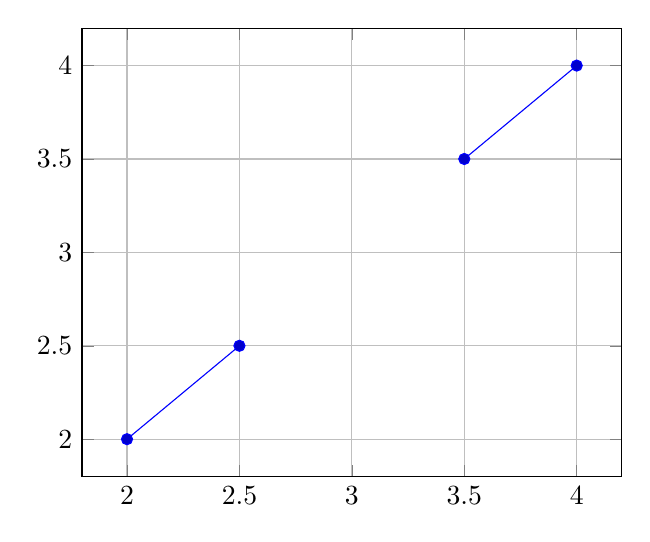
\begin{tikzpicture}
	\begin{axis}[grid=major]
	\addplot+[
		unbounded coords=jump,
		x filter/.expression={x+1},
		y filter/.expression={y==3 ? nan : y},
	]
	table {
	x y 
	1 2
	1.5 2.5
	2 3
	2.5 3.5
	3 4
	};
	\end{axis}
\end{tikzpicture}
\end{codeexample}
	
	The |x filter| is evaluated first. It can depend on |x|, |y|, and |z| whose values are the ``prepared'' coordinates: values which have been found after applying |x coord trafo| and any logarithms (for logarithmic axes).

	The |y filter| is evaluated as next. It can depend on |x| which is the result of |x filter|. It can also depend on |y| and |z| which have the same value as discussed in the previous paragraph.

	The |z filter| is evaluated as last. It can depend on |x| and |y| which are result of their respective filters. It can also depend on |z| which is the plain $z$ coordinate (as discussed for |x filter|).

	Defining filters by math expression is actually a special case of |x filter|, see below.
\end{\pgfplotsxykeylist}

\begin{pgfplotsxycodekeylist}{\x\ filter,filter point}
The code keys |x filter| and |y filter| allow coordinate filtering which are based on a \emph{single} coordinate. A coordinate filter gets an input coordinate as |#1| (on input, the same value is stored in |\pgfmathresult|), applies some operation and writes the result into the macro |\pgfmathresult|. If |\pgfmathresult| is empty afterwards, the coordinate is discarded. You can also set |\pgfmathresult| to |nan| or |inf| in which case the coordinate can be either discarded (if |unbounded coords=discard| is set) or the plot can be interrupted (the case |unbounded coords=jump|).

The |filter point/.code| filter allows filtering depending on all components forming a complete point ($x$, $y$ and $z$); it is described below.

It is allowed that filters do not change |\pgfmathresult|. In this case, the unfiltered coordinate will be used.

Coordinate filters are useful in automatic processing system, where \PGFPlots\ is used to display automatically generated plots. You may not want to filter your coordinates by hand, so these options provide a tool to do this automatically.

The following filter adds $0.5$ to every $x$ coordinate.
\begin{codeexample}[]
\begin{tikzpicture}
\begin{axis}[x filter/.code=
	{\pgfmathadd{#1}{0.5}}]
\addplot coordinates {
	(4,0)
	(6,1)
};
\end{axis}
\end{tikzpicture}
\end{codeexample}
Please refer to~\cite[pgfmath manual]{tikz} for details about the math engine of \PGF. Please keep in mind that the math engine works with limited \TeX\ precision.

During evaluation of the filter, the macro |\coordindex| contains the number of the current coordinate (starting with~$0$). Thus, the following filter discards all coordinates after the $5$th and before the $10$th.
\begin{codeexample}[]
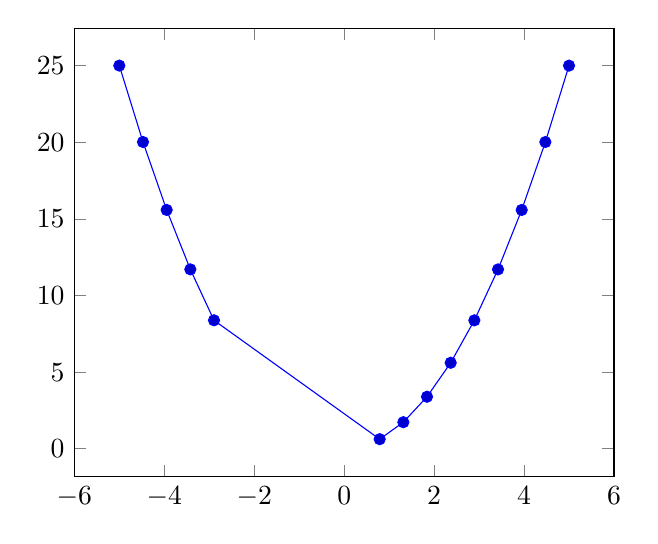
\begin{tikzpicture}
\begin{axis}[
	samples=20,
	x filter/.code={
		\ifnum\coordindex>4
			\ifnum\coordindex<11
				\def\pgfmathresult{}
			\fi
		\fi
	}]
\addplot {x^2};
\end{axis}
\end{tikzpicture}
\end{codeexample}
There is also a style key which simplifies selection by index, see below.

	\PGFPlots\ invokes the filter with argument |#1| set to the input coordinate. For $x$-filters, this is the $x$-coordinate as it is specified to |\addplot|, for $y$-filters it is the $y$-coordinate.

	If the corresponding axis is logarithmic, |#1| is the \emph{logarithm} (see |log basis x| and its variants) of the coordinate as a real number, for example |#1=4.2341|. In case the logarithm was undefined, the argument will be empty.

	The arguments to coordinate filters are minimally preprocessed: first, for logarithmic axes, the \emph{log} of the argument is supplied.  Second, any high level coordinate maps like |x coord trafo| (which may be used to map dates to numbers or string to numbers or so) are applied. In consequence, the |#1| argument is supposed to be a number. No further transformation has been applied.

	Occasionally, it might be handy to get the ``raw'', completely unprocessed input coordinate as it has been reported by the coordinate input routine. This unprocessed data is available in the three math parser constants \declareandlabel{rawx}, \declareandlabel{rawy} and \declareandlabel{rawz}. All these values are ready for use in filters (and some other methods influence plots as well). Note that |rawy| is to be used like a function without arguments, i.e.\ filters can employ it where math parsing is done. 
	
	An application could be to filter log values based on the normal scale:
\begin{codeexample}[]
\begin{tikzpicture}
\begin{semilogyaxis}
	\addplot+[
		restrict expr to domain={rawy}{1e0:1.5e1},
	]{exp(x)};
\end{semilogyaxis}
\end{tikzpicture}
\end{codeexample}
	\noindent The preceding example uses |rawy| to throw all samples outside of the range $[1,15]$ away.

	If key filters are invoked for |plot table|, access to the current row's data can be achieved using |\thisrow|\marg{column name} (and its variants). This includes all columns of the table.

	The |filter point| key is more technical. It doesn't take an argument: its arguments are given in terms of the |pgfkeys| variables |/data point x|, |/data point y| and |/data point z|. It may change its coordinates using |\pgfkeyssetvalue{/data point x}|\marg{new value}; access to variables can be accessed with |\pgfkeysvalueof{/data point/x}| or, if the argument shall be written into a macro, with |\pgfkeysgetvalue|. This filter is evaluated after the other ones.

	Note that you can provide different |x filter|/|y filter| arguments to each |\addplot| command. It seems there are only problems with the `|#1|' argument, and I haven't yet found out why. Please use |\pgfmathresult| in place of |#1| if you provide |\addplot[x filter/.code={...}]|.

	Note that coordinate filtering is also available for |mesh|, |surf|, and |patch| plots\index{mesh!Coordinate filtering}\index{surf!Coordinate filtering}. In this context, a |patch type| is drawn if and only if all its vertices have bounded coordinates. In other words: if one vertex of, say, a rectangle has been filtered away, the entire rectangle will be omitted. Coordinate filtering for |mesh| and |surf|ace plots has a further special requirement: the default for such plots is |mesh input=lattice|. If a coordinate filter silently discards a coordinate, the lattice will break and \PGFPlots\ will become confused. Consequently, coordinate filtering for |mesh| and |surf|ace plots always needs |unbounded coords=jump|, and any point which is filtered away should receive the value |nan| instead of an empty string (since empty strings will \emph{always} be discarded even in presence of |unbounded coords=jump|). Please see the reference documentation of |unbounded coords| and the example therein on page~\pageref{pgfplots:interrupt} for details about coordinate filtering and three dimensional plots.
\end{pgfplotsxycodekeylist}

\begin{pgfplotscodekey}{pre filter}
	Applied before |x filter|, |y filter|, and |z filter|.
\end{pgfplotscodekey}

\begin{stylekey}{/pgfplots/skip coords between index=\marg{begin}\marg{end}}
	A style which appends an |x filter| which discards selected coordinates. The selection is done by index where indexing starts with~$0$, see |\coordindex|. Every coordinate with index $\meta{begin} \le i < \meta{end}$ will be skipped.
\begin{codeexample}[]
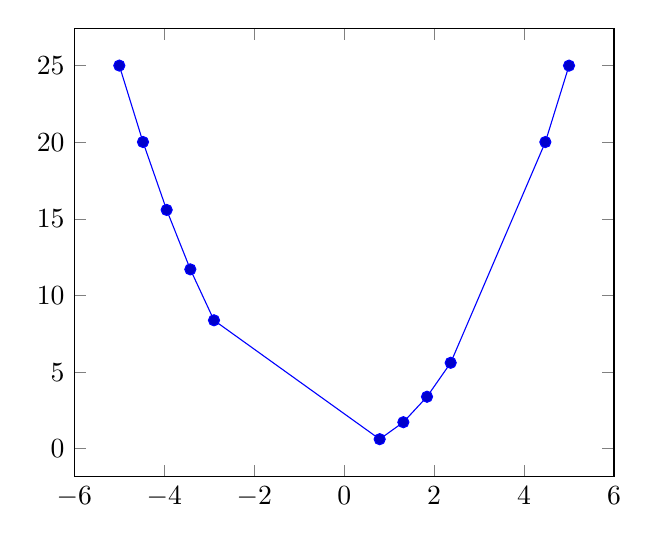
\begin{tikzpicture}
\begin{axis}[
	samples=20,
	skip coords between index={5}{11},
	skip coords between index={15}{18}]

\addplot {x^2};
\end{axis}
\end{tikzpicture}
\end{codeexample}

	\paragraph{Technical note}: this style usually applies to $x$ coordinates (i.e.\ it counts $x$ coordinates). In case you want to apply it to something like |hist/data| or |quiver/u|, you can 
	\begin{enumerate}
		\item append an asterisk `|*|' to the style's name and
		\item provide the target coordinate's name as first argument.
	\end{enumerate}
	For example, |skip coords between index*={hist/data}{2}| applies to |hist/data|.
\end{stylekey}

\begin{pgfplotskey}{each nth point=\marg{integer}}
	A style which appends an |x filter| which discards all but each $n$th input coordinate.
\index{Downsampling}

	This downsampling works fairly well. It can be used to reduce a huge amount of coordinates from an input file. In this case, you should also set |filter discard warning=false| to avoid repeated notifications about skipped coordinates and |unbounded coords=discard| such that \PGFPlots\ should silently forget any discarded points (rather than generated interrupted plots).

	Note that there is also a |mark repeat| style which applies the same operation to plot marks only.

	\paragraph{Technical note}: this style usually applies to $x$ coordinates (i.e.\ it counts $x$ coordinates). In case you want to apply it to something like |hist/data| or |quiver/u|, you can 
	\begin{enumerate}
		\item append an asterisk `|*|' to the style's name and
		\item provide the target coordinate's name as first argument.
	\end{enumerate}
	For example, |each nth point*={hist/data}{2}| applies to |hist/data|.
\end{pgfplotskey}

\begin{pgfplotsxykeylist}{
	restrict \x\space to domain=\meta{min}:\meta{max},
	restrict \x\space to domain*=\meta{min}:\meta{max}}
\label{key:restrict:x:to:domain}
	These keys append $x$ (or $y$ or $z$) coordinate filters to restrict the respective coordinate to a domain. 
	
	The versions without star (like |restrict x to domain|) will assign the value |-inf| if the coordinate is below \meta{min} and |+inf| if the coordinate is above \meta{max}. The starred versions (like |restrict x to domain*|) will truncate coordinates to $[\hbox{\meta{min}}, \hbox{\meta{max}}]$, i.e.\ they assign the value \meta{min} if the coordinate falls outside of the lower limit and \meta{max} if the value falls outside of the upper limit.

	For logarithmic axes, \meta{min} and \meta{max} are \emph{logs} of the respective values.  A variant which uses the non-logarithmic number might be to use |restrict expr to domain={\pgfmathrawx}|\marg{min}\marg{max}.

	The non-starred versions also set |unbounded coords=jump| which leads to interrupted plots.
\begin{codeexample}[]
\begin{tikzpicture}
\begin{axis}[
	restrict y to domain=-10:10,
	samples=1000,
	% some fine-tuning for the display:
	width=10cm, height=210pt,
	xmin=-4.7124, xmax=4.7124,
	xtick={-4.7124,-1.5708,...,10},
	xticklabels={$-\frac32 \pi$,$-\pi/2$,$\pi/2$,$\frac32 \pi$},
	axis x line=center,
	axis y line=center]

\addplot[blue] gnuplot[id=tangens,domain=-1.5*pi:1.5*pi] {tan(x)};
\legend{$\tan(x)$}
\end{axis}
\end{tikzpicture}
\end{codeexample}
\end{pgfplotsxykeylist}

\begin{pgfplotskeylist}{%
	restrict expr to domain=\marg{expression}\marg{\meta{min}:\meta{max}},%
	restrict expr to domain*=\marg{expression}\marg{\meta{min}:\meta{max}}%
	}
	Appends an $x$ coordinate filter which sets the $x$ coordinate to |-inf| if the \meta{expression} evaluates to something less than \meta{min} and to |inf| if \meta{expression} evaluates to something larger than \meta{max}.

	The starred variant, |restrict to domain*| assigns \meta{min} if \meta{expression} is less then the lower limit and \meta{max} if it is larger than the upper limit.

	The non-starred version also sets |unbounded coords=jump| which leads to interrupted plots.

	In contrast to |restrict x to domain|, \meta{expression} can depend on anything which is valid during |\addplot|, in particular |\coordindex| or table columns (|\thisrow|\marg{column name} and friends). The expression doesn't need to depend on $x$ at all.
\end{pgfplotskeylist}

\begin{pgfplotskey}{@restrict to domain=\marg{filter name}\marg{expression}\marg{\meta{min}:\meta{max}}\mchoice{0,1}}
	A low--level (technical) key which allows to apply the |restrict * to ...| features also to something like |hist/data|.

	For example,
	|@restrict to domain={hist/data}{}{0:1}{0}| applies the domain-restriction to the histogram-input |hist/data|. The final `|0|' means that it works in a similar way as the key |restrict x to domain=0:1|, i.e.\ it skips everything which is outside of $[0,1]$.  In a similar way, 
	|@restrict to domain={hist/data}{}{0:1}{1}| applies the functionality of |restrict x to domain*=0:1| to |hist/data|: it truncates values outside of $[0,1]$ to the domain's end-points.

	The \meta{filter name} is expected to be a coordinate name like |x|, |y|, |z| (or |hist/data|).

	The \meta{expression} configures an expression which will be used rather than the value of \meta{filter name}. It can be empty.

	The \meta{min}\texttt{:}\meta{max} are as described above.

	If the last argument is |1|, any coordinate outside of the allowed domain will take the domain boundary as value. If it is |0|, such a coordinate will get either |inf| or |-inf|.
\end{pgfplotskey}

\begin{pgfplotskey}{filter discard warning=\mchoice{true,false} (initially true)}
	Issues a notification in your logfile whenever coordinate filters discard coordinates.
\end{pgfplotskey}

You can find somewhat more on coordinate filtering in Section~\ref{pgfplots:interrupt}: ``Interrupted Plots''.
